% Tenplate for TAR 2014
% (C) 2014 Jan Šnajder, Goran Glavaš
% KTLab, FER

\documentclass[10pt, a4paper]{article}

\usepackage{tar2014}

\usepackage[utf8]{inputenc}
\usepackage[pdftex]{graphicx}
\usepackage{booktabs}
\usepackage{amsmath}
\usepackage{amssymb}
\usepackage{listings}
\usepackage{hyperref}

\title{Sentiment prediction in user reviews}

%VAŽNO: Zakomentirajte sljedeću liniju kada šaljete rad na recenziju
\name{Jakub Ziec, Marcin Trzcinski} 

\address{
University of Zagreb, Faculty of Electrical Engineering and Computing\\
Unska 3, 10000 Zagreb, Croatia\\ 
\texttt{jakziec@gmail.com}, \texttt{mrctrzcinski@gmail.com}\\
}
          
         
\abstract{ 
This document proposes a method and shows result of sentiment classification and rating prediction model for user reviews on a certain product from different doimains such as: books, dvds, ect. Each user review is classified as either Positive, or Negative. Additionally, the system is be able to predict the rating assigned to the product based on the review (i.e. on a scale from 1 to 5).
}

\begin{document}

\maketitleabstract

\section{Introduction}

The goal of this project is to build a sentiment classification and rating prediction for textual user reviews on certain products.  Reviews were taken from multiple domains, including books, DVDs, electronic devices etc.  The classification model was evaluated in terms of accuracy, precision, recall and F1-score. The rating prediction model was evaluated using a regression metric called Pearson correlation.



\section{Data prepatarion}

As we used three diffrent tools i.e. lingpipe in java program, libshorttext and libsvm, we preapared our raw input data\footnote{\texttt{\url{http://www.cs.jhu.edu/~mdredze/datasets/sentiment/domain_sentiment_data.tar.gz}}} in three diffrent formats. For the first one we used xml format and for others format required by used libraries. 


\section{Sentiment Classification}

For a classification problem i.e. deciding whether review has positive or negative sentiment, we chose two techniques: Naive Bayes classifier and support vector classification by Crammer and Singer. The first one we used as baseline.

\subsection{Naive Bayes classifier}

Naive Bayes classifier is simple probabilistic classifiers based on applying Bayes' theorem with strong (naive) independence assumptions between the features. The Bayes classifier is the function that assigns a class label $\hat{y} = C_{k}$ for some $k$ as follows:

\begin{equation}\label{eq:bayes}
\hat{y} = \underset{k\in\left\lbrace 1, .., K\right\rbrace } {\mathrm{argmax}} P(C_{k})\Pi_{i=1}^{n} P(x_{i} | C_{k})
\end{equation}
In our implementation we used \emph{Java} library \emph{lingpipe}. We represented document\slash review as \emph{bag of words} (\textbf{BoW}). We removed stop-words and removing all non-letter characters.

\subsubsection{Results}

The most frequent words given from our model for electronics domain for positive and negative training cases are shown in tables \ref{tab:mostFreqWordsPos} and \ref{tab:mostFreqWordsNeg}.

\begin{table}[ht]
\caption{The most frequent positive words}
\label{tab:mostFreqWordsPos}
\begin{center}
\begin{tabular}{ll}
\toprule
Word & nomber of occurrence \\
\midrule
i & 2721 \\ 
you & 915 \\ 
my & 859 \\ 
t & 519 \\ 
very & 339 \\ 
use & 323 \\ 
great & 311 \\ 
good & 310 \\ 
sound & 295 \\ 
these & 292 \\ 
your & 290 \\ 
just & 244 \\ 
quality & 231 \\ 
like & 231 \\ 
\bottomrule
\end{tabular}
\end{center}
\end{table}

\begin{table}[ht]
\caption{The most frequent negative words}
\label{tab:mostFreqWordsNeg}
\begin{center}
\begin{tabular}{ll}
\toprule
Word & nomber of occurrence \\
\midrule
i & 3078 \\ 
my & 827 \\ 
you & 711 \\ 
t & 673 \\ 
me & 311 \\ 
get & 276 \\ 
just & 272 \\ 
work & 255 \\ 
these & 253 \\ 
your & 236 \\ 
product & 226 \\ 
very & 226 \\ 
them & 217 \\ 
use & 215 \\
\bottomrule
\end{tabular}
\end{center}
\end{table}

The model for electronics domain gives following results:
\begin{equation}
\begin{split}
& Test Cases = 497 \\
& Correct = 324 \\
& Accuracy = 0.65191 \\
& Precision = 0.65060 \\
& Recall = 0.65322 \\
& F1 = 0.65191 \\
\end{split}
\end{equation}

\subsection{Support vector classifier by Crammer and Singer}

We decided to use libshortext library for support vector classification by Crammer and Singer. LibShortText is an open source tool for short-text classification and analysis. It can handle the classification of, for example, titles, questions, sentences, and short messages - The fast training and testing is built upon the linear classifier.

We used libshorttext in following manner:

\begin{lstlisting}[language=bash]
$ text-train.py -f -G 1 train_set
$ text-predict.py -f test_set model \
result.txt
\end{lstlisting}
Parameter -G 1 means that we using libshorttext with enable grid search (slightly better results than without). It uses no stopword removal, no stemming, bigram preprocessor options and binary feature representation.

\section{Rating prediction}

For raiting prediction we used support vector regression (SVR). The model produced by support vector classification depends only on a subset of the training data, because the cost function for building the model does not care about training points that lie beyond the margin. Analogously, the model produced by SVR depends only on a subset of the training data, because the cost function for building the model ignores any training data close to the model prediction.

In our solution we used libsvm library with following comend:

\begin{lstlisting}[language=bash]
$ svm-train -s 3 -t 2 -c 20 -g 64 \
-p 0.1 train_set
\end{lstlisting}

which means that we used epsilon-SVR regression with kernel function equal to $\exp(-\gamma*|u-v|^2)$, hyperparameter $C$ equal to 20, $\gamma$ parameter equal to 64 and $\epsilon$ equal to 0.1. For those parameters we obtain following results for electronics domain:
\begin{equation}
\begin{split}
& Mean\_squared\_error = 1.13938 \\
& Squared\_correlation\_coefficient = -4.00855e-15 \\
\end{split}
\end{equation}

\section{Demonstration program}

Our demonstraition program was written in \emph{Python 2.7} under \emph{Ubuntu 14.04.1 LTS}. It requires \emph{Java 1.8}, \emph{libshorttext-1.1} and  \emph{libsvm-3.20}.

\subsection{User Interface}

Our program has command line interface (see figure~\ref{fig:interface}).

\begin{figure}[ht]
\begin{center}
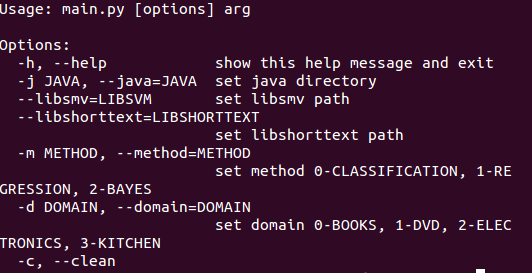
\includegraphics[width=\columnwidth]{help}
\caption{Command line interface}
\label{fig:interface}
\end{center}
\end{figure}

Example of using:

\begin{lstlisting}[language=bash]
sentiment-prediction/src$ python \
main.py -m 3 -d 0
\end{lstlisting}

will execute sentimental classificasion using Naive Bayes classifier and data from "books" domain.

An example output is show in figure~\ref{fig:output}.

\begin{figure}[ht]
\begin{center}
\includegraphics[width=\columnwidth]{output}
\caption{Program output}
\label{fig:output}
\end{center}
\end{figure}

\section{Conclusion}

How we can see Accuracy in vector classification by Crammer and Singer is about 12\% greater then in Naive Bayes Classifier. In naive Bayes classifier we used tokenizer which avoiding following english stopwords: a, be, had, it, only, she, was, about, because, has, its, of, some, we, after, been, have, last, on, such, were, all, but, he, more, one, than, when, also, by, her, most, or, that, which, an, can, his, mr, other, the, who, any, co, if, mrs, out, their, will, and, corp, in, ms, over, there, with, are, could, inc, mz, s, they, would, as, for, into, no, so, this, up, at, from, is, not, says, to. The results are a bit better then when we used tokenizer which taking into account every word but not so much how we expected
We suspect that results in SVR regression are not correct
the mean squared error and correlation coefficient seems to be ok but the results file contain the same output for every test data. We spend about 15 hours trying to repair it but without any positive effects. We were trying to scale test and training data, using  library with different parameters but each attempt was unsuccessful. We had not enough time to resolve this problem.

\section{References}
\url{http://www.cs.jhu.edu/~mdredze/datasets/sentiment/domain_sentiment_data.tar.gz} \\
\url{http://www.cs.jhu.edu/~mdredze/publications/sentiment_acl07.pdf} \\
\url{http://www.csie.ntu.edu.tw/~cjlin/libshorttext/} \\
\url{http://www.csie.ntu.edu.tw/~cjlin/libsvm/} \\
%\bibliographystyle{tar2014}
%\bibliography{tar2014} 

\end{document}

